\chapter{Introduction}

%Introduce the general area of interest that the contents of the review deal with, setting out any advancements and challenges of interest. Then introduce more fully the specific topic addressed in the review and you can then to go on to state any main aim or objectives to be met. Say very briefly what is to come in the layout of the review. Note: the Introduction should include general references to back up the points made.
% Establishing the field
%Definition:
%What are the Olympic classes sailing?
%How are the competitions setting  up?
%What does position and direction means?
%What time steps are you referring for the wind forecast, which sizes?

In recent years the integration of new technologies on training programs of professional athlete have been increased. Not only to enhance their motor skills, and to prevent injuries but also to obtain better results with a minimal time and in a more efficiently process. For example, the use of information that specify the conditions or parameters that delivers the best results to win have gained more popularity within the sport community. The involvement of science like kinesiology \cite{sjogaard2015science}, movement science; and engineering is not only concentrated in the athletes furthermore in the elements and factors that can not be controlled by them but of those which impact their results. One of these sports is sailing where athletes have to guide the boat under different weather conditions and where time is critical to win the race.\newline

During sailing races such as coastal, inland waterways and lakes athletes are not allow to get any information from coaches during the race; for this reason, their preparation and training is not only physical. During training they acquire skills to anticipate the weather changes and at the same time maneuvers to improve the performance of the boat. \\
%For example, a well know competition and classes are the Olympic sailing competitions which take place on coastal and improvements on the boat are not allow. \\

In this section the research problem, its relevance and the objectives are going to be presented. For this, a brief definition of Olympic sailing classes and courses are going to be explained followed by an explanation of the information considered by the coaches and athletes to plan the strategy before the competition take place which most of the time this refer to the weather forecast. These data provides a framework to setup the assumptions and limitations used in this research.
\\

\section {Olympic Sailing} \label{sec:olympic classes}
The Olympic Sailing Classes are characterized by the rule of one-design boat. The intention of this is to leave out the influence of technology on the results and focus on the abilities of the athlete to perform effectively; for this reason, the scope for many researches is on the athlete only. The figure \ref{fig:olymp_cla} shows the names and categories of the currently classes that the International Federation of sailing define as Olympic Classes. The list is subject to changes and review after every Olympic cycle. The dinghy is the boat with more classes, the differences between them relies on the dimensions of the boat and sail. This dimensions are determine by the number of crew members,1 or 2, and gender. This is one of the reasons why this research is going to use the dinghy as a reference boat, another reason is due to its similarity physically and mathematically with yachts.\\

\begin{figure}[ht]
\centering
 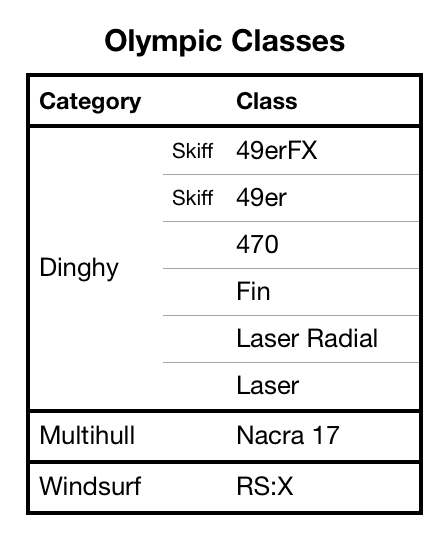
\includegraphics[width=0.32\textwidth]{olym_classes.png}
  \caption{Olympic classes \cite{sailoly}.}
\label{fig:olymp_cla} 
\end{figure}

The competition on each class stand for many races and days where the configurations of the course varies according the environmental conditions. In each race, points are given according is arrival position; the faster, the lower score. The winner is the one with the lowest score. Under this competing format athletes and coaches confront distinct scenarios for which they take different decisions at the start line. One of these decisions refers to the initial sailing direction. The importance of it is related with the configuration of the course.\\

\subsection{Competition Course}\label{tracks}
The most common form of a sailing competition is the fleet racing where all participants race around a course and start at the same time along the start line. Here not only the reaction time to compete is important but the direction that allow the maximum speed that could be attained. Usually two different types of courses took place for the Olympic classes. Figure \ref{fig:trap_c} shows the singular trapezoid course which is defined by a separate start and finish line and 4 points around (buoys); these 6 elements define the legs of the competition and the first leg is usually the longest one and it is running against the wind.
The trapezoid course is the most completed format course, the other formats are a partial representation of it, considering only some leg already represented in the trapezoid course.\\
%The other course is the windward/leeward, figure \ref{fig:wl_c} this is simply a two-leg race orientated in such way that the first leg is sail against the wind (called a beat) and the second leg is sail with the wind (called a run). If boats are sailing neither with nor against the wind, the leg is called reach. 

\begin{figure}[ht]
  \centering
  \subfloat[Trapezoid Course ] {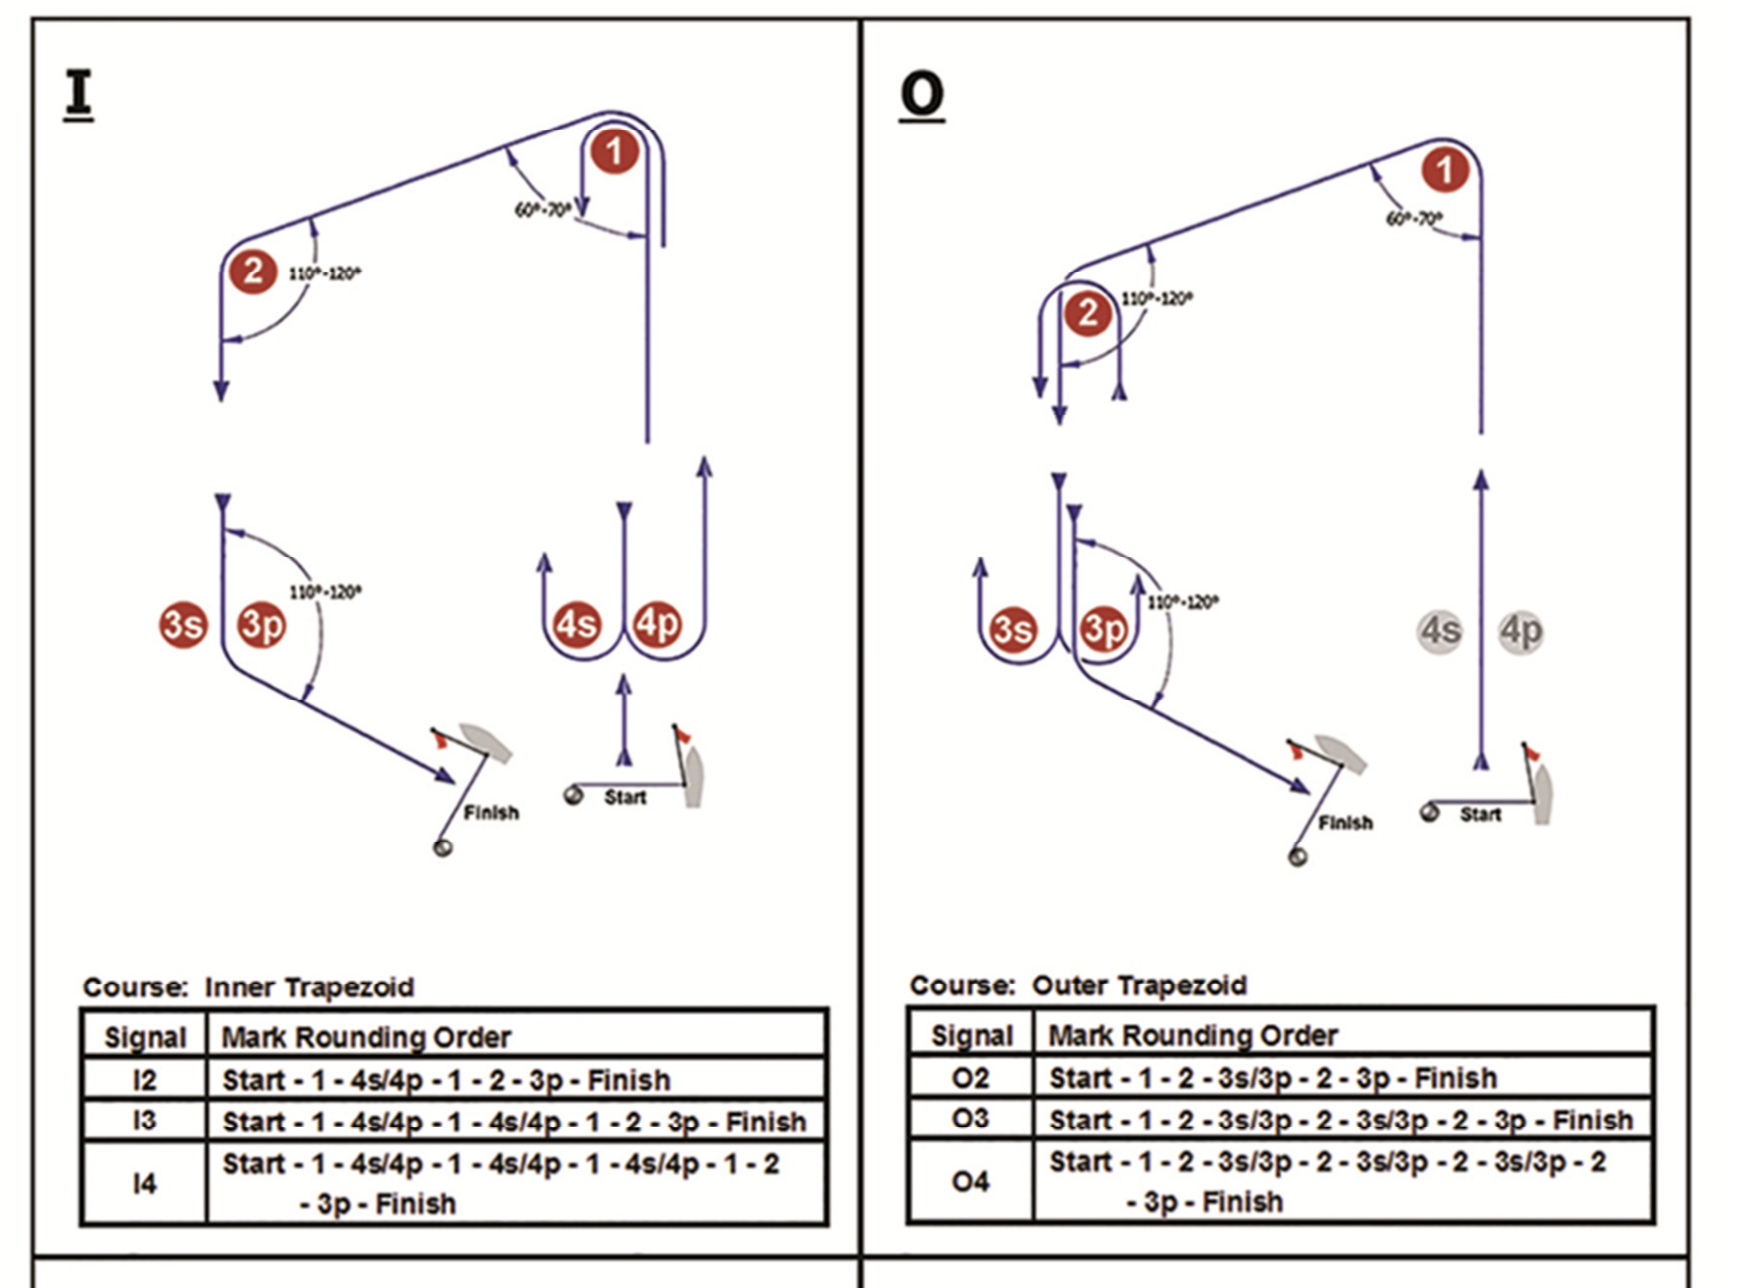
\includegraphics[width=0.53\textwidth]{trap_course.png}\label{fig:trap_c}}
  \hfill
  \subfloat[Windward / leeward course] {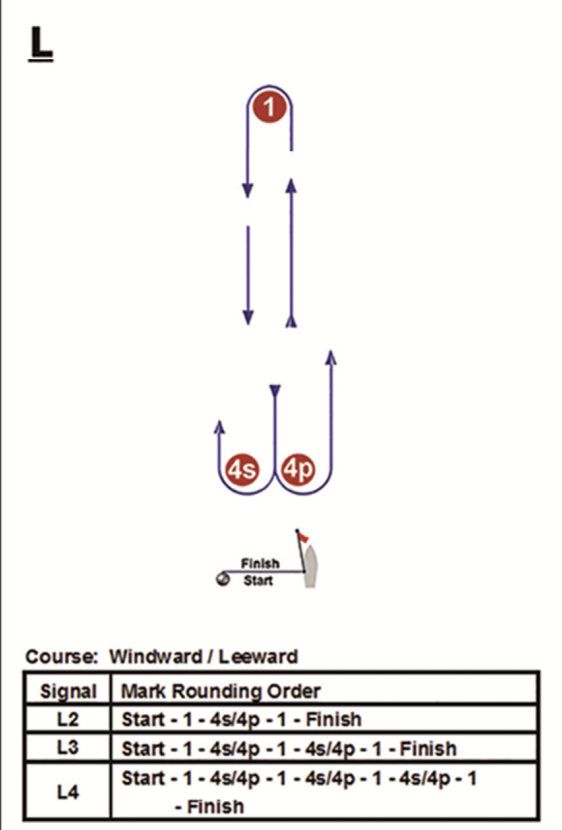
\includegraphics[width=0.25\textwidth]{l_w.png} \label{fig:wl_c}}
  \caption{Types of courses \cite{instr_rio}.}
\label{fig:typecourses} 
\end{figure}
Because the the first leg is the longest one and it runs against the wind 

\cite{race_pol} regulates and define the courses characteristics and conditions to race, these are subject to changes every 4 years. The length and angles of each leg are defined in such way that the course could be completed in maximun 1 hour and the trapezoidal course can be contain in a grid size of 2km by 2 km.  Another consideration is the area of the course,  which most of the time is expressed in nautical miles (nm). Figure \ref{fig:olymp_areas_rio} is an example of how the sailing areas are defined by a circular area, within this circle the trapezoid should be located. Furthermore, the wind conditions refers to the average wind speed in addition to its shift direction.\\
%The race will not start if the average wind speed is less than 4 knots or more than 25 knots over the entire course. However, the maximum wind shift allowed is 10\deg. 
If wind conditions are not meet the race could be delay, and if the race has already started it is possible a change on the course or an abandon of the race \cite{race_pol}. It is clear how important is the wind for sailing; however to understand how it interacts with the boat and the athlete it is important to know the physics of sailing. \\

\begin{figure}[ht]
\centering
 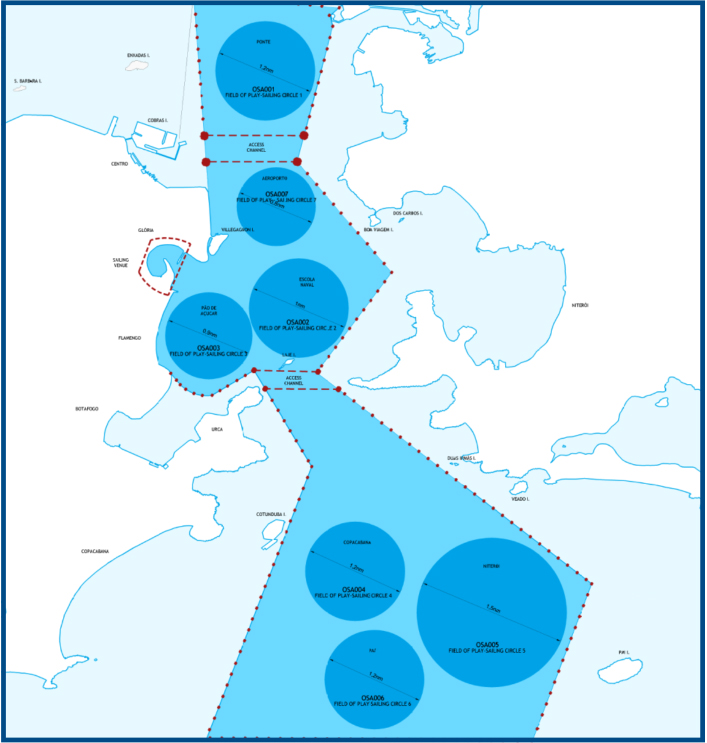
\includegraphics[width=0.65\textwidth]{16_OG_RaceAreasNOR.jpg}
  \caption{Sailing Races Areas. Olympic Games Rio 2016 \cite{instr_rio}.}
\label{fig:olymp_areas_rio} 
\end{figure}

\section {Sailboat Physics Model} \label{sailphysics}
%The objective of this section is to present the problem jargon and basic concepts of sailing.
%Sailing boats are propelled mainly by wind, however they displace through the water; in other words, sailboats move through 2 different fluids: water and wind.The mechanics of sailing have been know since 1950's.  Marchaj in 1979 review them and add information which is still being used for yacht design \cite{marchajaereo1979}. 
%Figure \ref{DOF} shows the 6 fundamental types of motion or degrees of freedom (DOF) for boats with the names and axis where they are developed: 3 translations and 3 rotations.  

%The static and dynamic balance of any type of boat is based on Newton's second law. \\
:  in static condition, the equilibrium is reach when the summation of all the forces and momentum equals zero; while in a dynamic situation, as when the boats moves, it is the velocity that leads this equilibrium.
%\begin{figure}[ht]
%\centering
%  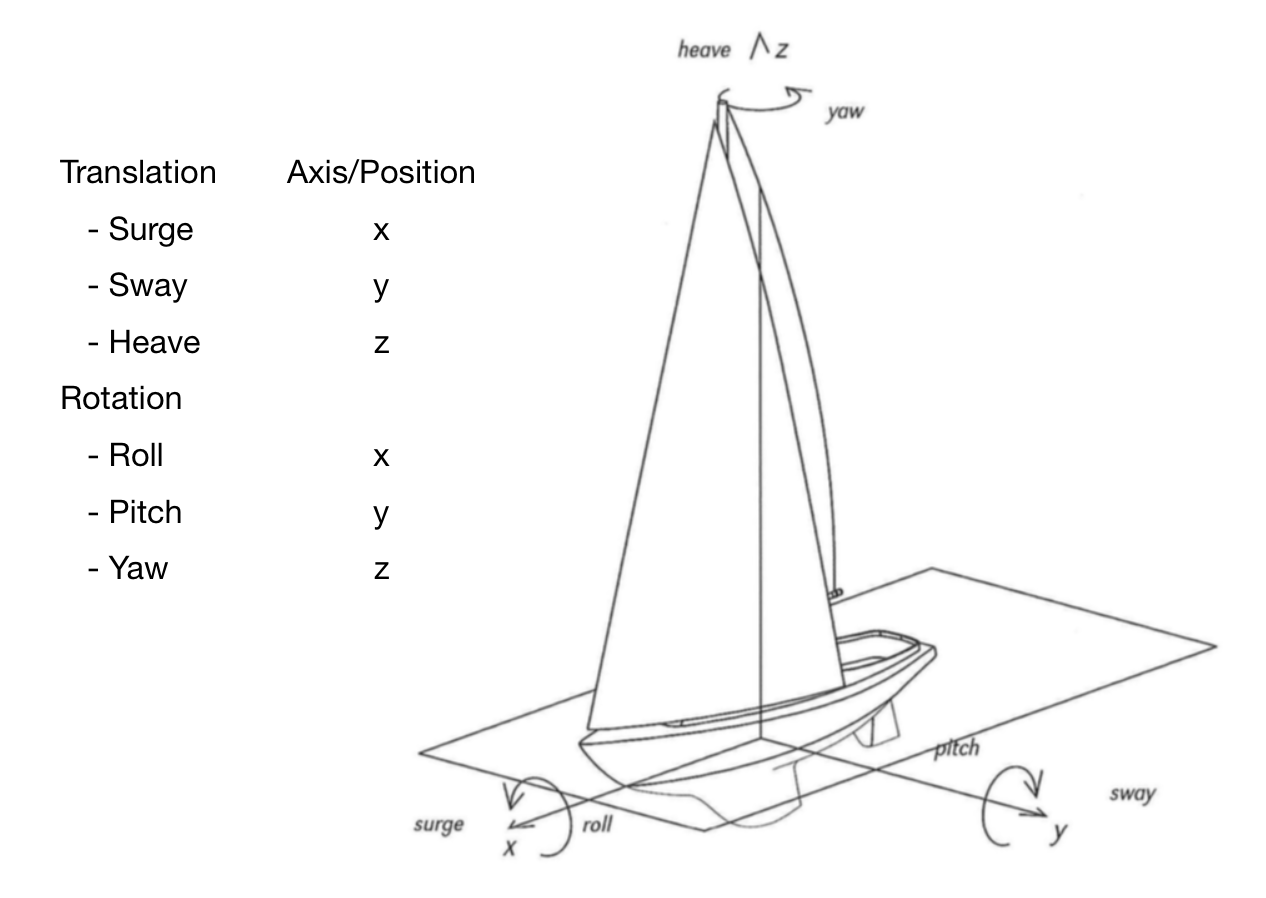
\includegraphics[width=0.7\linewidth]{dof_foss_modif.png}
% \caption{Degrees of freedom of a boat, clockwise reference system xyz %\cite{fossati2009aero}. }
%\label{DOF}
%\end{figure}
%Since both fluids are influenced by atmospheric factors, these creates a time-dependent environment to model. 
Therefore, the dynamics of the sailboat is determine by its interaction with both fluids, while the control is given by the seamanship through the rudder and sail angles. Consequently, the seamanship interact with aerodynamic and hydrodynamic forces which at the same time generate resistances.
%Because the sail boat interact between two fluids not only they generate forces but also resistances in one or both mediums.
%it is important to know how the elements are named and which words are related with specific manoeuvres.  This simple concepts, will help you to understand how the equilibrium is generated in the static condition, what elements interacts on it and how it is conserved when the sailboat moves from one point to another. 

\\
These mechanism determine the equilibrium conditions that define how the sailboat moves\cite{fossati2009aero}.  As an example of this, the maximum speed of a sailboat depends on the wind and current velocities and the heading of the sailboat with respect to the wind. The relation of this variables is non linear and it is represented by the Velocity Prediction Polar (VPP).\par

%As consequence of the forces interaction, the velocity of the boat can be represented in the so called velocity triangle, see figure.
The steady-state equilibrium of the boat, as a consequence of the forces interaction during motion,  is reach via velocities. The wind, current and boat velocities interaction is represented with the velocity triangle.  As we can see in figure \ref{vel_triangle}, the relation between wind and boat velocities, result in another 2 velocities; the apparent wind velocity  and speed made good,  also know as velocity made good (vector notation). It is important to explain that the velocity of the current is considered in the boat's velocity, equation \ref{eq_vel}; where  is the true wind velocity respect to the boat,  $c_b$ is the current velocity respect to the boat, $\alpha$ is the sail angle and \textit{V} is the velocity vector. According \cite{larsonprinciples}, the velocity made good \textit{(VMG)} provides useful information to understand where is the sailboat on the space is and how is its motion. Therefore, this triangle have to be considered for any type of analysis.
%% Include equations here 
\begin{equation} [ht]
\label{eq_vel}
\begin{aligned}
V_{aw} & = V_{tw,b} - V_{c,b} - V_{boat} \\ 
VMG &=  \mid V_b cos \alpha  \mid 
\end{aligned}
\end {equation}
vaw and its direction $( \alpha_{a_w})$ are highly important because it is the velocity perceived by the moving sailboat and its is given by the difference between the wind and the boat; if the boat is moving in the same direction as the wind then the apparent velocity increase. 
%% If height exceed width, then the effective sail area is A=pi h/4. The area of the air used in our calculations depends on the height of the sail, this is explained in the prandt and . The force of the boat is given by  Fboat= Fwind cos (a sail-app wind) cos (avw- sail-app wind). If the boat is in downwind condition veq=wind vel/( 1+ (beta)^0.5 ) and beta = drag factor / (density air * Area sail)

\begin{figure}[ht]
\centering
  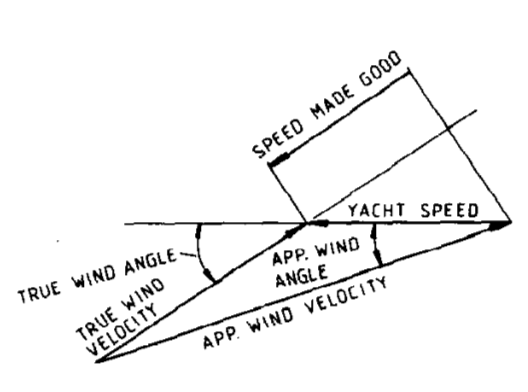
\includegraphics[width=0.45\linewidth]{Larsson_triang_vel.png}
 \caption{Velocity triangle  \cite{larsonprinciples}. }
\label{vel_triangle}
\end{figure}
 
Philpott  in \cite{philpott1993yacht} explains how different elements of the boat, see figure \ref{sailboat_terms}, interact with the surroundings and how they are used to control and attain the equilibrium during motion. The main elements of the sailboat, including wind, currents and waves were grouped in 3 categories or factors, each of them affect the equilibrium in a different way.
 \begin{enumerate} \label{factorphil}
% \setlength \itemsep{0em}
 \item Environmental factors; such as wind and current intensity and direction,
 \item Design factors, dimensions that characterize the type of boat. 
 \item Control variables, variables affecting by the sailmanship
 \end{enumerate}
 
 \begin{figure}[ht]
\centering
  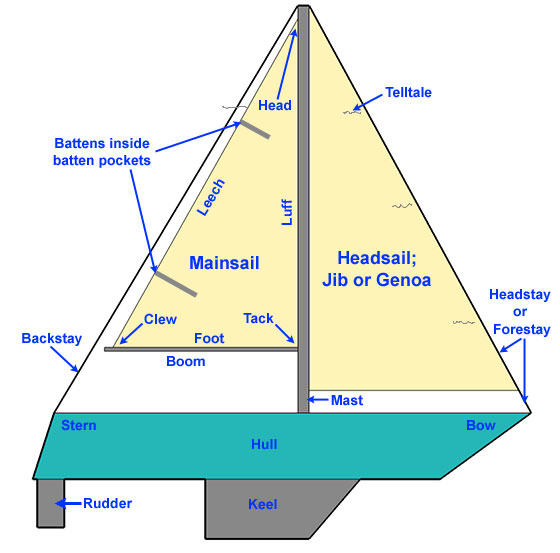
\includegraphics[width=0.47\linewidth]{sailboat_terms.jpg}
 \caption{Common sailboat terms \cite{sailboat_terms}. }
\label{sailboat_terms}
\end{figure}
 
\cite{philpott1993yacht}  explain that in order to steer a boat the sailmanship has control the angle of the rudder, which interacts directly with the current, the direction obtained by adjusting it is called heading and these two generate forces that influence the boat to \textit{yaw}. Due to the wind direction, mainly; the boat slip sideways or in other words it has leeway. The difference in course comparing with the heading is expressed as leeway angle. The sails adjustment or trim during sailing is called \textit{reefing}, this last helps the sailmanship to control the wind intensity.  The wind over the sails, generates a force and an angle called \textit{heel angle}, this decrease the driving force. Under those circumstances, a moment is generated and to neutralize it, the sailmanship generates a \textit{righting moment} by standing on the windward side of the boat to produce it. A graphical representation of the interaction of these forces is  found in \ref{forces_m}.  As a result of these forces, the velocity could be optimal or not. \cite{larsonprinciples} relates the factors and forces proposed in\cite{philpott1993yacht} in terms of forces and resistances, indicating how the dynamics of each of the mediums, water and air,  interact to keep the balance (and be capable to maximize the boat's speed)  in three items, as indicated below; 
\begin{itemize}  \label{milgramforces}
 \setlength \itemsep{0em}
\item Aerodynamic driving forces = Hydrodynamic resistance;
\item Aerodynamic side force = Hydrodynamic side force;
\item Aerodynamic heeling moment=Hydrodynamic (static) righting moment.
\end{itemize}

% \begin{figure}[ht]
%\centering
%  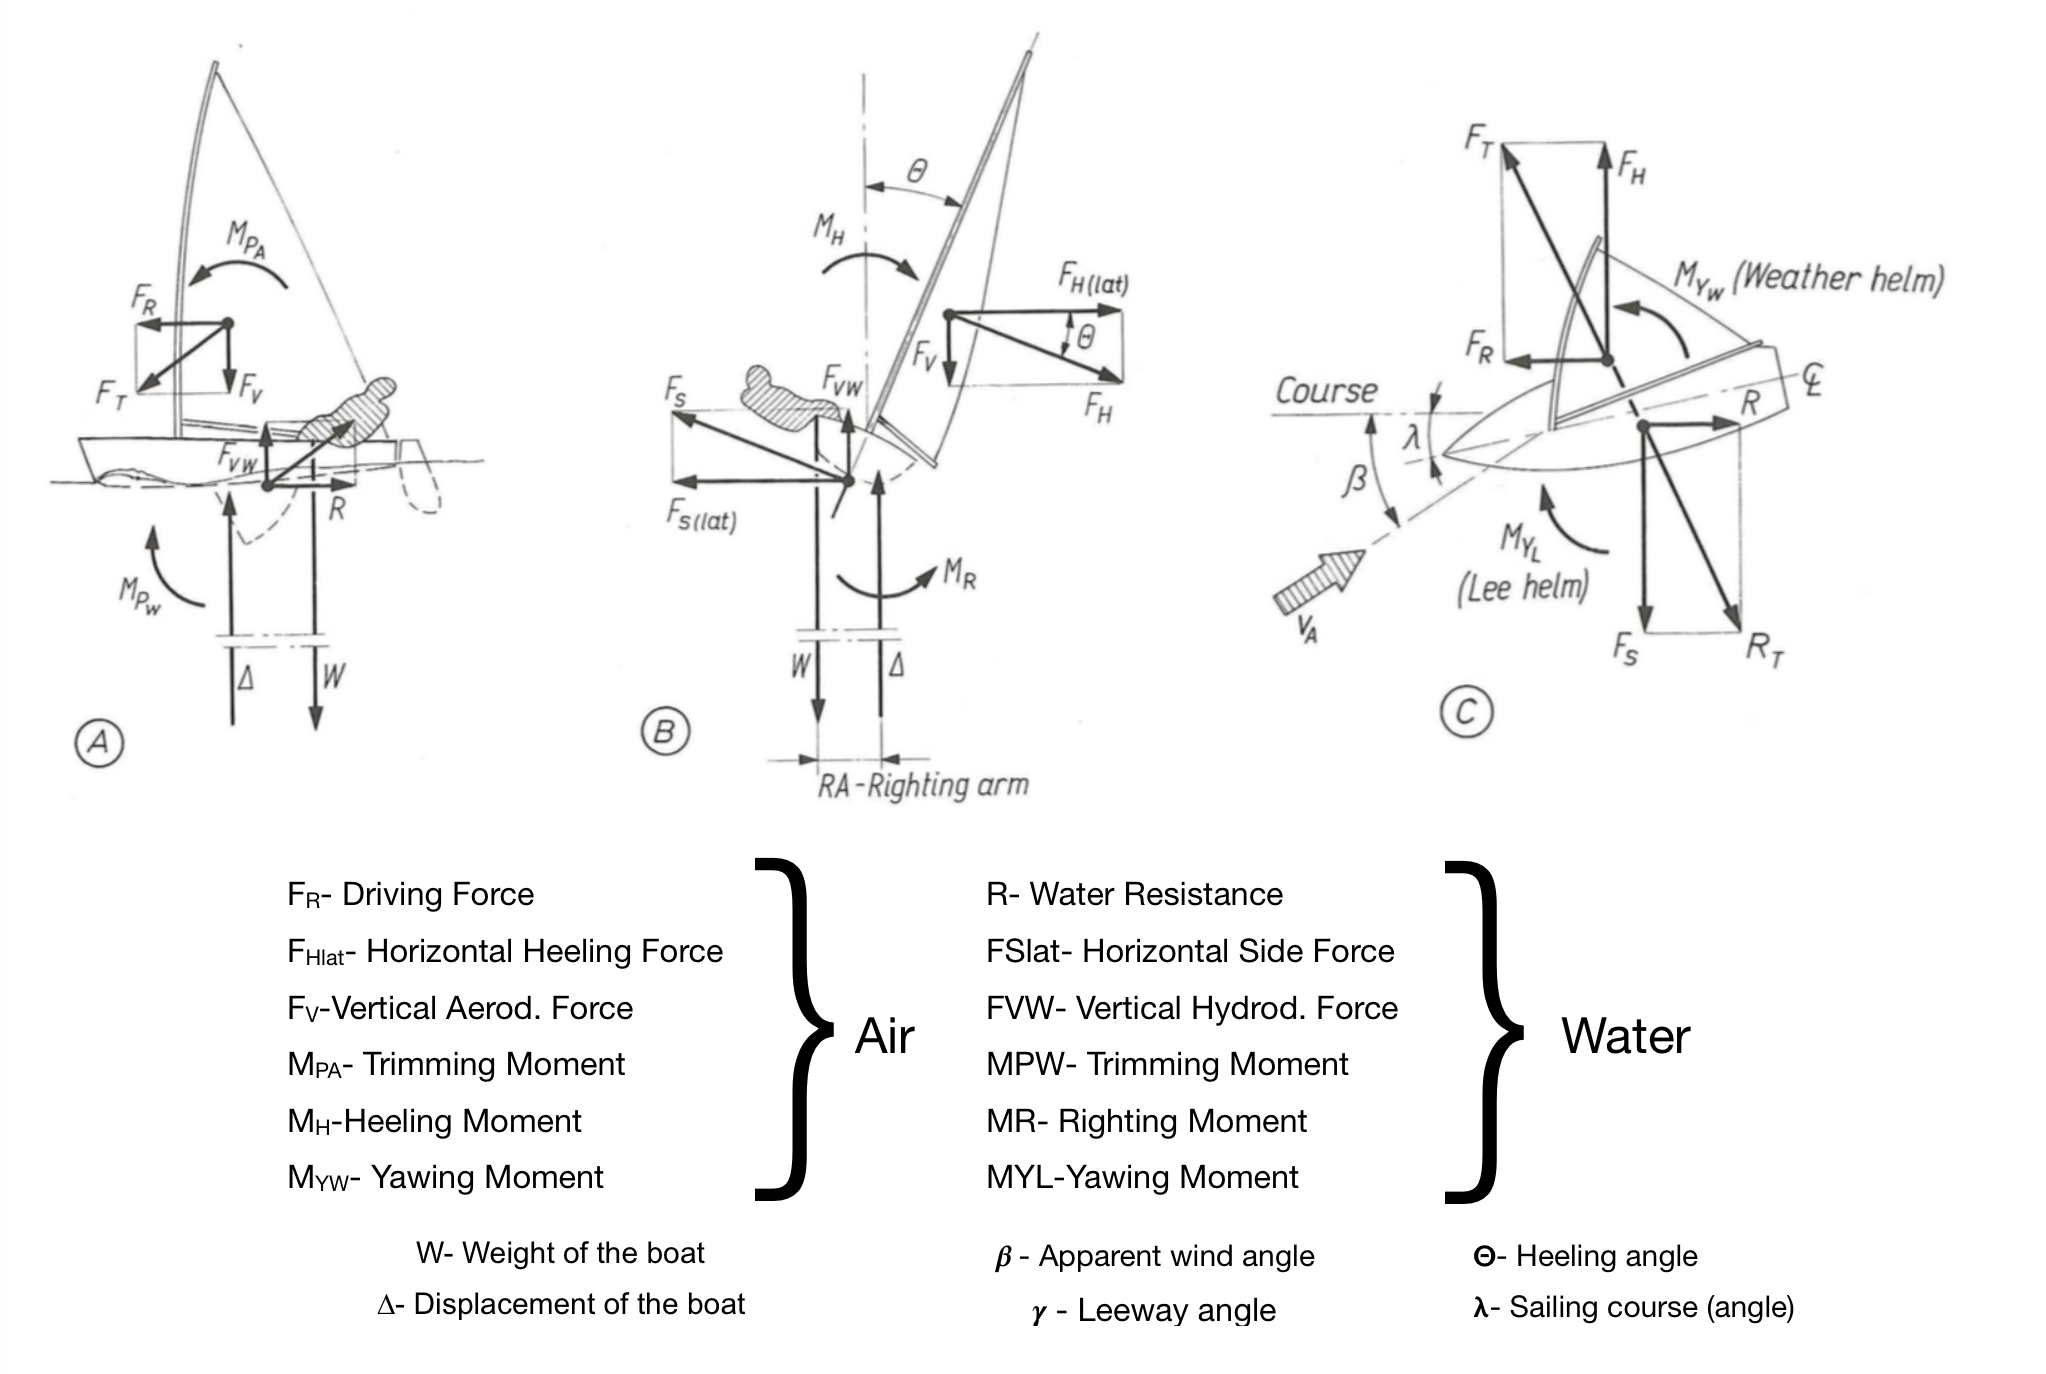
\includegraphics[width=.97\linewidth]{marchaj_forces.png}
% \caption{Equilibrium of forces and moments in steady-state sailing condition %\cite{marchajaereo1979}. For details see Appendix \ref{forces_equations} }
%\label{forces_m}
%\end{figure}

An important assumption made by  \cite{philpott1993yacht} and \cite{larsonprinciples} to keep the analysis of the boat in 2 dimensions is that vertical forces are in balance always same as the pitching moment. In rough water, however the pitching motion reduces the speed and it is compensated by both mediums, the aerodynamic and hydrodynamic forces. Another consideration refers to the wind, the force it generates over the sails is applied at  the center of effort on them which is assumed to be located at 40\% of the mast height \cite{philpott1993yacht}. \par

The direction of the boat respect to wind no only determines the apparent velocity but also the type of maneuvers and trajectory that it most follow. If the boat is moving in upwind direction, this means that it is beating the wind, the boat has to move following a zig-zag pattern.  Each change on the heading direction is known as tack; therefore it is a tacking maneuver the ones that allows the sail to move against the wind. \\ \cite{denny2009float} explains that there is a transitory stage during a tacking maneuver, where the sail switch from one side to the other at each turn.  The transitory state happens when the bow is directly upwind, here the sails are positioned parallel to the wind direction to reduce the wind resistance. Meanwhile, it is the momentum which is carrying with the displacement most of the time with some contribution made by the rudder, if this transitory state takes too long, the boat will finish without propulsion; what is known as in the irons. \\According \cite{denny2009float}, coming about is the maneuver that includes tacking and the transitory state described before.  To avoid this transitory state, and make use all the time of the sails, the sailmanship could perform another maneuver knows as jibing, which is also knows as wearing about, see figure \ref{manoeuvers}.\par 

\begin{figure}[ht]
  \centering
  \subfloat[Tacking Manoeuver.]{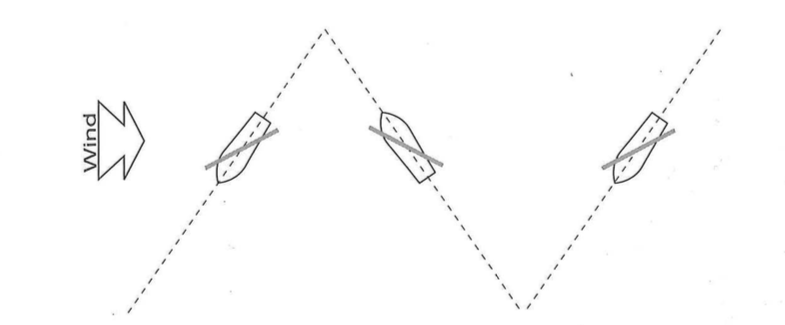
\includegraphics[width=0.4\textwidth]{tacking.png}\label{tacking}}
  \hfill
   \centering
  \subfloat[(a) Tacking and coming about;(b) jibing and wearing]{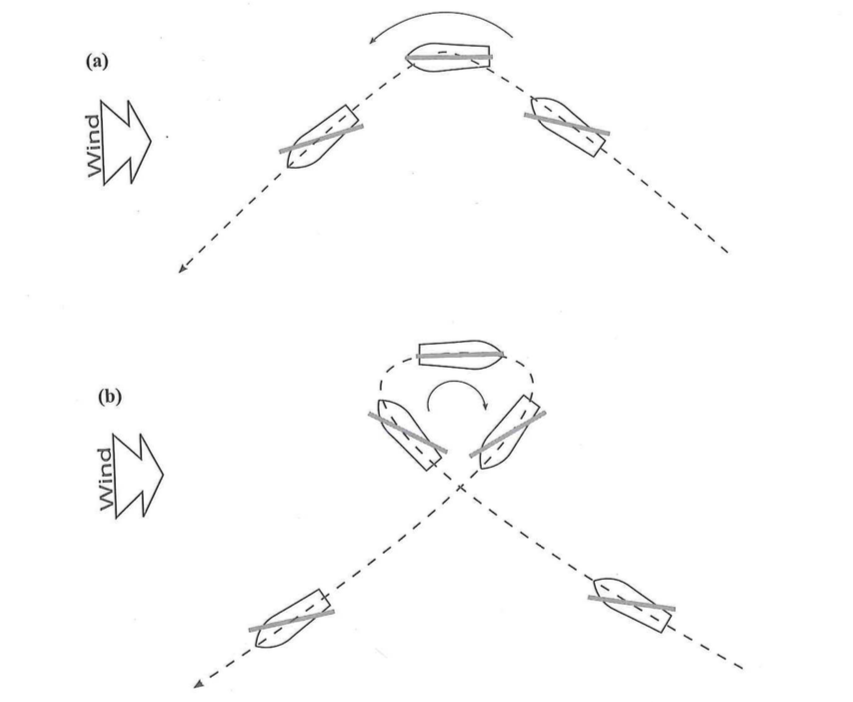
\includegraphics[width=0.4\textwidth]{tackandjib.png}\label{tack_jib}}
  \caption{Common maneuvers for sailboats \cite{denny2009float}.}
\label{manoeuvers} 
\end{figure}

In sailing, the motions with respect to the wind define the type of manouvres to execute.  Since the sailboat can not displace towards the wind, tacking manoeuvers are perform. These type of paths are described as zig-zag patterns that can be started on the left- or on the right-hand side. Another condition is dictated when the boat is displaced in the same direction as wind. These conditions shows that feasible paths are asymmetrical\cite{dolinskaya2012optimal}. Because athletes are not allow to get any information or feedback from coaches, preparation is crucial. The information of how to course must be deliver before competition and it have to be trained. Another element to consider is the no-go zone where the propulsion is null or not enough to displace the sailboat\cite{yang2011control}.


To determine the sailboat velocity, between the wind direction and its course, that can be reach under different environmental conditions, wind angle and magnitude, scientist developed in 1979 a velocity prediction program (\textit{VPP}). This program according  \cite{larsonprinciples}, use the equations for static equilibrium and information about the hydrodynamic, aerodynamic and stability properties of the sailboat.  The solution is given by  the forces mentioned in \ref{milgramforces} and the apparent wind velocity and direction. By using the VPP not only the maximum sailboat speed can be obtained including the direction, for the sailboat and sail, that should be follow but also the angles that should be avoid \cite{yang2011control}, to stay away from the irons. Because VPP plots are symmetric only half of them are usually represented, see figure \ref {vpp_diag}. 

\begin{figure}[ht]
  \centering
  \subfloat[VPP plot for true wind for true wind angles from 0º to 180º and true wind speeds from 4 to 10 m/s \cite{larsonprinciples}.]{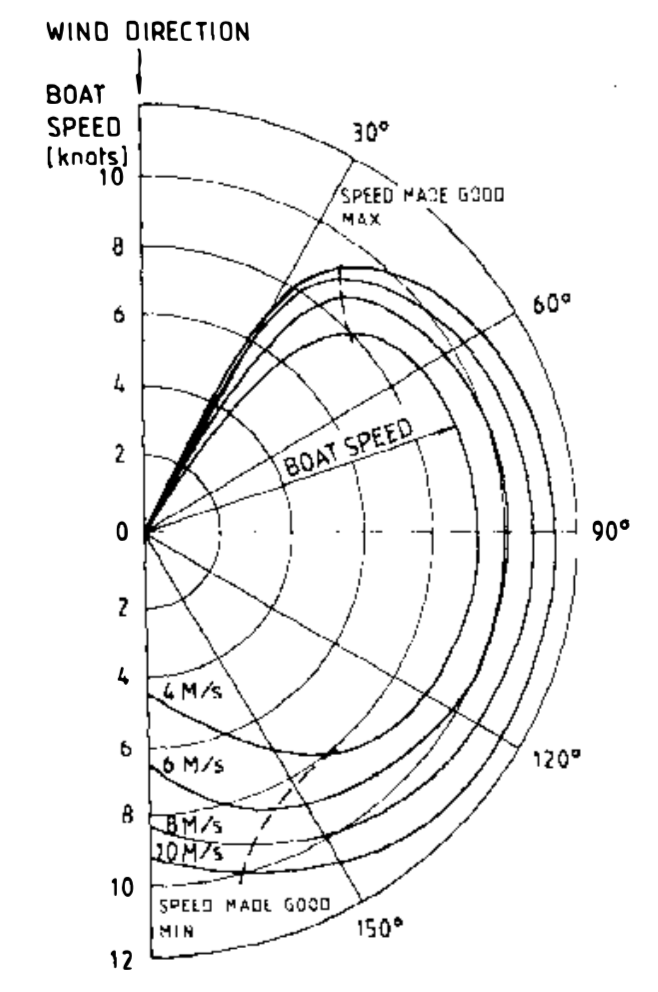
\includegraphics[width=0.37\textwidth]{vppLarsson1990.png}\label{typ_vpp}}
  \hfill
  \subfloat[Polar Curve of the Propulsion System \cite{yang2011control}(Full VPP representation).]{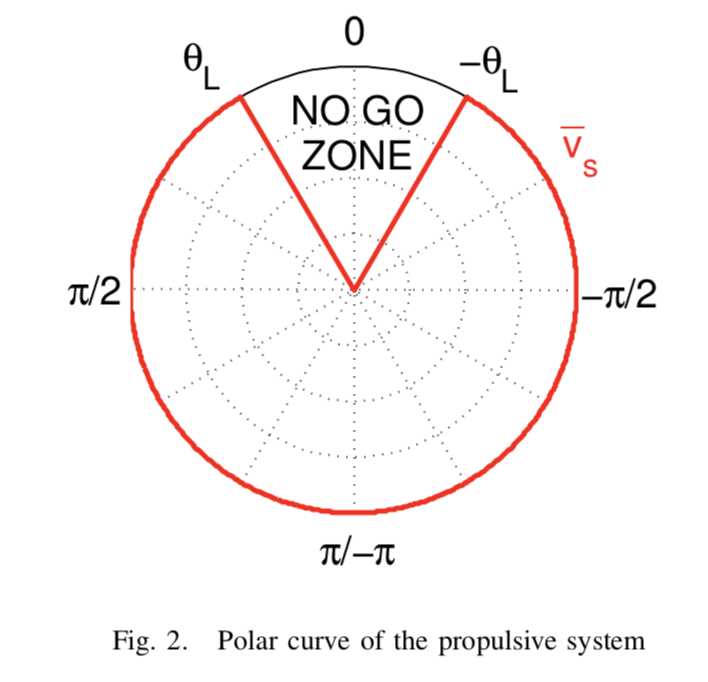
\includegraphics[width=0.5\textwidth]{no-go_zone_yang.png}\label{no_go_zone}}
  \caption{VPP diagram}
\label{vpp_diag} 
\end{figure}

%The solution of  the VPP predict the sailboat speed for any wind and sailing angle between the wind direction and the course of the boat.
%\subsection {Olympic Classes}

%The Olympic Classes of Sailing are characterized by the rule of one-design boat. Since 1924 the tendency  has been in the direction of smaller one-design sailboats with fewer crew members. The intention of this is to leave out the influence of technology on the results and focus on the abilities of the seamanship to perform effectively. Currently, the International Federation of sailing define 8 classes;  one windsurfing board, one multihull and six variants on the dinghy. 
\\The focus on this research is on laser classes which use a dinghy, a small type of boat, and it contemplates two classes.  %meaning one hull and a centreboard or daggerboard, which is an adjustable fin primarily used to stop the boat and moving sideways through the water
The difference between laser classes refers to the sail area.The laser has a sail area about $7.06 m^2$  and it is competed by men; while the radial has a sail area about  $5.76 m^2$ and it is competed by women.

%\begin{figure}[ht]
%  \centering
%{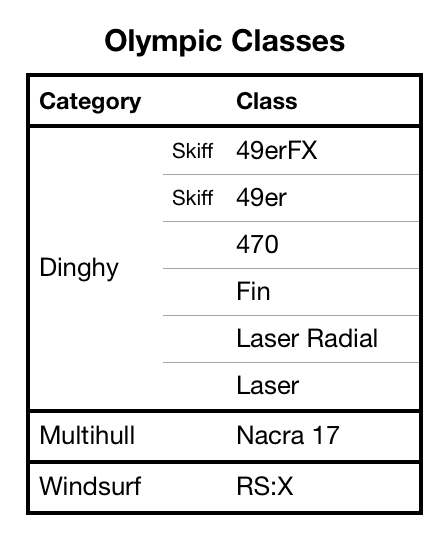
\includegraphics[width=0.32\textwidth]{olym_classes.png}\label{olymp_c}}
%  \hfill
%  \subfloat[Laser Class] {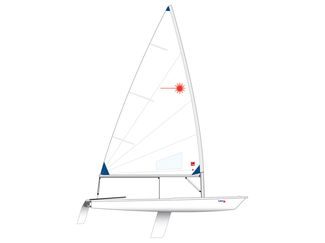
\includegraphics[width=0.55\textwidth]{laser.jpg} \label{laser_c}}
%  \caption{Olympic classes \cite{sailoly}.}
%\label{laser} 
%\end{figure}





Much of the research found refer to yachts competitions. Where the boat design can be modified however this is not the only difference, the shape and dimensions of the course differ significantly. For example, the Volvo Ocean Race is and offshore competitions that stand for months with a total distance between legs of 45,000 nm; due to the format, the wind and other weather conditions can change significantly.  Due to the size of the competition different approaches are borrowed from logistics and nautical sciences in in order to plan the strategy and path to win the race. This is not the case of the Olympic classes. Despite the fact that both type of boats, dinghies and yachts are governed by the sames physics behind 







\\ 
\\
The focus on this research is on laser classes which use a dinghy, a small type of boat, and it contemplates two classes.  %meaning one hull and a centreboard or daggerboard, which is an adjustable fin primarily used to stop the boat and moving sideways through the water
The difference between laser classes refers to the sail area.The laser has a sail area about $7.06 m^2$  and it is competed by men; while the radial has a sail area about  $5.76 m^2$ and it is competed by women.








 The information of how to course must be deliver before competition and it have to be trained.

%Importance:
%Why the comparison of the time steps is important?
%Is the start direction significant to minimal time path?
%What are the conditions of this?
%Why current softwares cannot be used for this purposes?
%Method:
%How the  wind forecast time step size are going to be compare? (Experiments/Simulations)
%Specifications:
%What wind model forecast  is going to used? 
%Which olympic sailing class are going to be used on the test?
%Where the simulation is going to be taking place?
%Assumptions:




\subsection{The optimal-path problem for Laser Classes}
 %This section is an in depth review of a particular area(s) and/or methods that you will require to complete your project. This could, for example, be particular theories, (mathematical) tools or solutions from other related areas that could be used to solve the problem. Discuss the different solutions/methods, are there disadvantages to using them? Why are they appropriate? What other areas can be used to augment the solutions in order to make them more suitable.
%Note: This is the main part of a review and should be highly structured in a consistent manner, in presenting the various works of interest and showing understanding of how it all links together. Ensure you cluster the literature appropriately and that papers are consistently related to each other, avoiding stand alone papers.
%In the project proposal the literature review highlights the gap in the knowledge that you have identified. While in this literature review you discuss (an aspect of) what you are going to use in order to fill the gap in the knowledge. What areas are to be combined in order to cover the gap in knowledge.
This section will provide the information about the methods and different approaches and considered for the modeling of the minimal time path for races of Olympic classes; in other words, the optimal path.  As Sjøgaard explained \cite{sjogaard2015science},  sailing is considered an interdisciplinary sport that deals and interact with the environment and multiple factors that provide different information that models the decision-making for the tactics used not only to compete but also to win.  Different disciplines like logistics, operations research, robotics and maritime have been study the optimal path problem. 
Most of the time, the objective of these disciplines is  the optimization of a cost function, related to the destination arrival time, fuel consumption or fleet efficiency. In the other hand, the weather is a variable that not all the time has been considered and when it is different mathematical methods has been used. %\\Not to mention, the computational effort variable which is going to consider during the evaluation of the literature. %As a matter of fact, the keywords used for this literature research were logistics, sailing, yachts, maritime, optimal path, weather and operations research. 
At his point, it is important to remember that wind is the main propulsion system for sailboats, althought the optimal path problem is not  new.\\
%Despite this, the application of all of them is limited when it refers to sports, more specific to short courses as the one for the olympic classes. 
Yacht competitions, like the Volvo race has been study longer than olympic classes; in general most of the research work developed until know for sailboats and sport is related to yachts. As a matter of fact, the research performed on dinghies, particular laser is limited. It is the on robotics field and autonomous vehicles where most of the research works for dinghies sailboats has found; consequently most of the methods used belongs to control engineering. %  On the other hand, the researches on optimal path for wind propelled sailboats on short courses is also limited, since robotics, system and control  and automated vehicles are the specialties that lead them.
\\
The intention to understand how the problem has been defined, its limitations and assumptions guide us to organize this section in the next way;  the first parts refers to the techniques used for trajectory optimization problem, the optimization of the minimal path-time; the second part treats with the methods used for uncertain weather. The last part refers to the differences between yacht and dinghy, because most of the work is done on yachts, and time, therefore velocity, is more important than distance, VPP and sails models must been adjusted.
\par %Sailing races for Olympic classes are developed during one hour as maximum and its know that delays occurs, so even if the weather could be predicted accurately, tha model should not \par
%to figure out this problem and its solution 

\subsubsection{Model: Optimal-Path for sailing}

As mentioned in section \ref{sailphysics} the sailboat depends mainly on the wind to move and to increase or decrease its velocity, in addition to the disturbances on the wave and currents.  The sailmanship accounts these effects and information to trim the sail and rudder angle to achieve its destination.  In competition this adjustments are governed by maximum speed or minimal time, rather than the shortest distance. Then the optimal path is the one that meet next criteria: finish the course with a minimal time. \par
%The problem of the optimal for vessel has been approached by different perspectives or subjects; like logistics,  focus on maritime routes with the objective to reduce costs,  and in other cases to effectively use of  the fleet; robotics and autonomous vehicles have also review this topic not only for ships but also for underwater vehicles. 
The main methods and techniques used for the optimal path problem are related with operations research, by using dynamic programing and minimization of  the objective function, while for robotics, different control engineering techniques are used. Not to mentioned, the modified on the course as a consequence of feedback data; coming from sensors or other external systems.  In this way the uncertainty of the weather is reduced. 

%The problem in most of the literature found is defined also as a path planning, one of the reason is because data can be updated during the course either by a regional sensor or on-line measurement and the second is due to the fact that random and unpredicted events could happen and change the course leaving the decision of the direction to the sailmanship while the destination point(s) remain fix. The shape made by the destinations points not always has a trapezoid shape and the wind conditions on each leg is not as relevant as for competitions, besides the length of the course could stand for days, week or even months. 
%In this section the review is made on how the problem is solved in different subjects and what are the constraints and assumptions made on each.

%\subsubsection{Logistics and Operation Research Methods}
The optimal path problem most of the time has been related with the shortest path commonly found in logistics as networking optimization, both areas highly related with operations research and robotics. As in logistics the target location is known, and even when the networking optimization is included in the geometrical domain, because the shortest path, \textit{Euclidean} shortest path, is founded inside a polygon \cite{mitchell2000geometric}. The shortest distance objective doest comply fully to our problem,  first because a point located in upwind direction from the sailboat can only be reach with tacking maneuvers and second because traveling longer distances in a faster speed  compensate for shortest distance courses at a lower speed, this condition is considered in \cite{dolinskaya2012optimal} as direction-dependency, and as anysotropic medium in \cite{dolinskaya2012path}. In the case of vessels mentioned in \cite{dolinskaya2013fastest}, the algorithms developed used calculus of variations and optimal control theory most of the time. According \cite{kelly2015transcription} in general this problems are solved by using on of the next types of algorithms.  The election of one of those algorithms depends on the dimension of the system, number of variables, stability and effort to implement and initialize \cite{kelly2015transcription}; in addition to the accuracy and convergence of the solution. \par 
 \begin{itemize}  
\item Dynamic Programming: Solve Hamilton-Jacobi-Bellman Equations over the entire state space.  
\item Indirect Methods: Transcribe problem then find where the slope of the objective is zero.
\item Direct Methods: Transcribe problem then find the minimum of the objective function. 
\end{itemize}

As Philpott explain in \cite{philpott2001optimising}, dynamic programing (DP) not only breaks the problem in stages but also defines a set of state variables; as a result, each stage can be linked to the previous results, after this the next stage can be determine, it can say that the optimization is made in a recursively manner.
%The essential feature of dynamic programming is that it divides a problem into a set of linked stages, each of which depends on decisions made in the previous stages. The effect of all previous decisions is encapsulated into a set of state variables that are used to determine the optimal decision at the current stage. The determination of the optimal decision for each possible set of state variables is made recursively, typically starting with the optimal decision at the last stage of the problem
In all the works found it from Dolinskaya ,\cite{dolinskaya2012optimal}, \cite{dolinskaya2012path}, \cite{dolinskaya2013fastest},\cite{dolinskaya2012time} and \cite{dolinskaya2009optimal} DP was used to account the direcction-dependency of the medium. In the other hand, in \cite{mitchell2000geometric},  when the approach is the \textit{Euclidean} shortest path the different methods can be use, even when it includes the velocity on the objective function or in the 
Hence, the optimal path problem can be solve by using different mathematical techniques, and the election of one of them depends on the design variables defined. One of these variables, for sailing races is the weather which is related with the wind  and current and these can be constant or time and position dependent, because of this it is necessary to discretize the time and space by defining a proper grid size. How coarse or fine it is will depends on the convergence of the solutions and its accuracy, this concept is know as the granularity, the larger the more time it requires to compute a solution. Because  each point in the area sailing is describing by some data.% which the state of the analyzed area. % These conditions as mentioned in \cite{allsopp2000optimal} by adding uncertainty to the model therefore to the solution of the optimal path. % include brief mention of Raboud and the uthos of papers considering in this sections, like a resume o end paragraph of the introduction.
%These initial decision affects both conditions and it is also determine by the initial guess. At the same time, the initial guess could arrive to local minimum solutions which should be evaluated to identify how constant it is, in case of other local solutions or even breaking points where the solution can not be obtained. \par 
%Considering the observations made by Kelly, the focus of this research are made in direct methods mainly and dynamic programing or hybrid systems since the boat behaves in a different form in turns and upwind/downwind condition 
\subsubsection{Consideration to the Direction-Dependance for path development}
The dependancy of the optimal path related with the location of the vessel and weather dependent on time was elaborate in \cite{dolinskaya2012optimal}.  Here the anysotropy of the medium was accounted. The algorithm proposed use the DP recursive modeling in way that the computation effort is smaller compared with other algorithms. The model discretize the space using intermediate nodes. %This nodes were included because the problem statement includes the use of radars or other devices to measure  or gather information within the \textit{radar visible region}. The path is determine at the begining and later adapted with the information recollected.
In the case of the Olympic classes races the adaptation of the path is made by the athlete. However the algorithm consider the feasibility of the speed base on its location, which is something that can be used for the development of the algorithm of the Olympic classes races. \par 
%In \cite{dolinskaya2013fastest} the algorithm proposed is based  mainly in the shortest distance approach and not  on the maximum speed attain; however, it accounts for the anisotropy behavior of the media also, $AB \neq BA $.  Another  assumption used in this research is that the speed function is homogeneous in time and space. The methodology proposed accounts for obstacle-free and obstacle-avoiding domains; where the straight trajectory can be approximated by a close zig-zag pattern to it. This pattern serves to avoid the obstacles or restricted regions and are represented as polygonal shapes. The properties of the speed and their convexity velocity polar diagram  was used to adapt the visibility graph search method. The relevance of this works is related with the use of VPP to determine the optimal path and how the properties of the speed were accounted. Here, the shape of the VPP is different compared with the common shape of sailboats.
%Additionally  a number of theorems and preposition were defined to find the optimal path not only in convex regions but also in a non-convex, this last shape is closer to the one VPP diagram of sailboats. The most relevant preposionts found it were: preposition 3.1 which express the percentage reduction of time,  that can be obtain by following the optimal path  rather than a straight course. Besides it was acknowledge that the structure of the velocity function is important to determine if the optimal  travel time is hold by a straight line or not, also the fastest path could be not unique. Moreover theorem 3.4 accounts for situations where the speed is equal to zero meaning that there are conditions where the  trajectory is not feasible. % this conditions are valid only if "the linear path attainable region (LPAR) is convex", \cite{dolinskaya2013fastest}. 
%Here also has included the convex characteristic of the VPP diagram; once the convexity premise is relax, a new condition is incorporated by means of bounds, where the domain of the speed function changes from $[0, 2\pi]$ to $[-\pi, 3\pi]$ and this is expressed int  theorem 3.5. %\cite{dolinskaya2013fastest}.
%\par

%Dolinskaya in \cite{dolinskaya2012time} , also adjust the previous method proposed in  \cite{dolinskaya2013fastest}, and it use as baseline the Dubins car problem  (Dubins 1957). Considering that sailboats have a speed polar diagram which is not convex and the minimum turning radius they can accomplish not to mention  the direction-dependent of the wind, anisotropic medium \cite{dolinskaya2012time}; the turning radius in and anisotropic medium for a sailing boat is not constant, this dynamic behaviour add complexity to the model. However, the optimal path and the turning radius can be express by alternating a sharpest-turn following and a straight line segment two times a finished by another sharpest turn. By using optimal control theory, it was possible to derive a condition for optimization and establish that the minimum-turning radius depends on the vehicle speed and heading angle. The state of the system is defined by $(x(t),y(t),\theta(t))$. 
%\par
%The model of  \cite{dolinskaya2012time} describes the dynamics of the system using differential equations that account for the velocities of the previous variables and include boundary conditions for the initial, final and  zero position. Within the explanation and setup of the system it was recognize that a right turn end in a different point compared with the left turn and its time could be different, so the minimum time path problem was broken into a set of scenarios translated into sub-paths that meet all the constraints imposed. Because the optimal path on sailboats depends on the characteristics of its speed polar plot and some of this conditions define the shapes of the sharpest-turn curves the unique solution for this type of problem was analyzed on a case-by-case bases. These cases set the constraints that figure the optimal and unique solution of the system. The paper also highlight the fact that without a minimum-turning radius limitation the optimal path is formed by two straight lines each at specific headings (angles). \par

%Similar to \cite{rabaudoptimal} , in \cite{lolla2012path} the algorithm proposed considered time dependent flow fields, to move from one point to another which is applicable mainly for autonomos underwater vehicles (AUVs). The method is based on the use of level set methods, where a set points of a function acquires a constant value, and it could be represented as \textit{"wavefront"} or isocountour line, so the space or area and time have to been discretize, and at every step-time the value of the function is calculated. This method is a Hamilton-Jacobi approach and it requires that the vehicle has a constant speed to cross the velocity field of the flow. Geographical constraints are expressed as mathematically points where the velocity of the flow is zero, most important the computational effort grows linearly and geometrically, this last depends on the spatial dimension which according the authors allow us to have a reasonable time to find out the solutions. \par   
A different approach based on the VPP diagram was developed in \cite{philpott1993yacht}. Here the focus is on maximising  "the component of the velocity in the direction where the wind is coming from". This method seeks among all the possible trajectories that could cross the final destination and find the angle where this happens. The problem is solved by using dynamic programing where the taking maneuvers are given by  weighting the amount of sailing in a specific wind condition and the remaining  sailing in it, in other words by comparing the time expended in a particular direction with the remaining time to reach the objective. The method was tested with random starting points and the taking manoeuvres; however it was mentioned that some starting point makes the method to fail, since the model is non-linear it can be said that there are conditions  where the solutions are unfeasible. 


%\subsubsection{Geometrical Optics Approach}
In \cite{rabaudoptimal} the method proposed use approached in geometrical optics. 
%Another method to find the optimal path was proposed by Rabaud \cite{rabaudoptimal}, with an approached used in geometrical optics.  
Here was acknowledge that in sailing competitions the optimal path  could be the longest trajectory and its depends on weather conditions, so no matter the distance or how long is the trajectory until it delivers the minimal time to move from point A to point B. To do that the problem was formulated as equation \ref{rabaudmintime}.
\begin{equation} \label{rabaudmintime}
\begin{aligned}
T_{AB}=\int_{A}^{B} dt=\int_{A}^{B} \frac{dl}{v}  \\
\end{aligned}
\end{equation}
Because the VPP diagrams, the speed diagrams for sailboats, show that different angles can result in lower velocities  and that they are not even convex functions. Therefore, its behavior is not isotropic, in addition boats can not sail directly against the wind. However a point in that condition it is possible to reach by following a zig-zag pattern.\\
The envelope of the VPP diagrams were found in \cite{rabaudoptimal} similar with the Wulff construction used to predict the shape of a crystal. This construction is a function that relates an angle $\theta$ with the Gibbs free energy,$\gamma (\theta)$.  %Hence  $\gamma (\theta)$ is the inverse of the crystal growth speed in the direction $\theta$ whereas $V (\theta)$ is the boat velocity.  
In both cases the velocity depends on an angle and their plots are convex envelopes.  The model developed is based on the isochrones method used in geometrical optics which are called wavefronts. These wavefronts have circular shapes and each is the source of the next wavefront. Under this approach, the method proposed, in \cite{rabaudoptimal}, obtain the optimal path using
%Rabaud proposed an method to obtain the optimal path for sailing where 
%The isochrones of a sailing boat are analogous to the wavefronts of geometrical optics, the speed diagram playing the role of the inverse of the refractive index. The isochrone construction method corresponds to the Huygens construction for light wavefronts, where each point of a wavefront is considered as a source of circular waves
%he includes 
a wind field that depends on time and position \bm{$W(r,$}t\bm{$)$}. The method determine a curve at any time of the largest distance that can be reach in any direction between 2 points. The VPP diagram and the wind field provide the information of the position that can be the be attain in any direction $theta$ after a time interval. \\
\begin{equation}
\label{reach_position}
\begin{aligned}
\Delta t: \bm{r} =\bm{V}(\theta) \Delta t \\
\end{aligned}
\end{equation}
The wind intensity between the initial point and the isochrone curve $W(\bm{r,+ \Delta t})$,  is the one corresponding to the boat velocity on the VPP diagram.
%It is based on the determination at any time of the curve of the largest distances reachable in any direction from the initial position of the boat.
The isochrone curve at time $\Delta$t is made by join all the attained positions given by the full range of $\theta$. % and its shape is the convex envelop. 
To disregard variations on the predicted weather it was recommended to make $\Delta$t as small as possible.\\
This process is repeated until the curve made by  $\textit{t}+n\Delta t$ reaches the final position. Then the minimum-time path between A and B is determined by the normal trajectory that connect each isochron. The maximum speed corresponds to the direction of $\theta$ obtained by the VPP diagram, in this form the trajectory along $\theta$ direction is related with the maximum speed represented on the VPP at that same direction. \\   The conclusions of \cite{rabaudoptimal} mentioned the importance of the forecast weather to obtain and accurate path and its uncertainty  which could be approached by "adding stochastic noise on the data" \cite{rabaudoptimal} . 
\\
%A observation made is that the $\Delta$t must be small enough neglect time or spatial variations of the predicted weather. 
%Dolinskay 2008
The method proposed by Rabaud \cite{rabaudoptimal} is based on the enveloped formed by the isochrone and the maximum velocity provided by the VPP. 
The envelop shape of the VPP used in \cite{rabaudoptimal} was explained in detail by \cite{dolinskaya2009optimal}.This type of shapes represent a feasible region where a vessel can moves in a straight line in a period of time from the origin; and it was called     \textit{linear path attainable region} for point (0,0)" \cite{rabaudoptimal}. Even when the paper refers to vessel and not sailboats, many concepts can be apply, since the main idea stands for both type of boats.  This region is constrained also by not feasible heading directions  and bounds defined by operational constraints and under certain conditions it is possible to find more than one path with the minimum travel time. Moreover, it was mentioned that voluntary speed loss due to turns or changes on the heading direction results in new feasible regions which might not be completely convex and therefore a new method should be use under this circumstances. Additionally, changes either in the weather or in the time can be relaxed by representing them as stationary obstacles.\\
Until now,  the method proposed in  \cite{rabaudoptimal} and \cite{philpott1993yacht} are similar in the sense that they are based on the VPP. The discretization used is different however both researches show the importance of the weather.  In this point it is important that even when the solution could be represented by a polygon shape its discretization must be determined carefully to not finish with a problem with infinite points to evaluate as mentioned in \cite{mitchell2000geometric}.  \cite{rabaudoptimal} uses an important observation made in \cite{dolinskaya2013fastest} where polar diagrams of the vessels were characterized according its convexity shape. This shape can arrive to optimal solutions which are not unique. Because of this a  case-by-case analysis were performed to set  or impose the limitations so an unique solution can be determine.
%An optimal path for a vehicle is highly dependent on the characteristics of its speed polar plot and the shapes of the sharpest-turn curves and can only be further analyzed on a case-by-case bases
%Without making assumptions regarding the structure of either the direction- dependent speed function nor the minimum-turning radius function, we establish the system’s controllability, demonstrate the existence of an optimal path, and invoke optimal control theory techniques to derive a necessary condition for optimality.
 %Unmanned aerial vehi- cle (UAV
 % homogeneous speed function. 
%traditionaly the euclidean shortest-path is used to find a solution. 
%\subsubsection{ Control Engineering Methods for Path Optimizartion}
%ADD KElly constrast with Mitchell
%even when the objective is to minimize a cost function, or reduce the travel time.   
%\par % review next paragraph once the definition of the track is completed and the rules for definng the route
%The types of tracks and how they are defined were explained in secction \ref{tracks}. Since  windward-leeward courses are common, Xing....
The courses of sailing competitions on Olympic classes include upwind and downwind conditions, indeed some of the legs have to conducted as a windward-leeward course. Considering this Xing \cite{xing2012path} proposed an algorithm to optimize the path under these 2 conditions. If a local solution is found and the course can be discretize, the summation of the solutions will provide the global solution. In \cite{xing2012path},  the local optimal solution is figured out by a heuristic search, a fuzzy conceptual method to developed  the algorithm assuming that wind, waves and current are constant.
Despite this research is focus on the optimal with a wind dependent on time and location. It is important to review how this type of problems has been approached  and if it can be modified or adapt for this purpose.\\
%% heuristic search:  is a technique designed for solving a problem more quickly when classic methods are too slow, or for finding an approximate solution when classic methods fail to find any exact solution. This is achieved by trading optimality, completeness, accuracy, or precision for speed. In a way, it can be considered a shortcut. is a function that ranks alternatives in search algorithms at each branching step based on available information to decide which branch to follow.
%% fuzzy conceptual method:A fuzzy concept is a concept of which the boundaries of application can vary considerably according to context or conditions, instead of being fixed once and for all.[1] This means the concept is vague in some way, lacking a fixed, precise meaning, without however being unclear or meaningless altogether.[2] It has a definite meaning, which can be made more precise only through further elaboration and specification - including a closer definition of the context in which the concept is used. A fuzzy concept is understood by scientists as a concept which is "to an extent applicable" in a situation. That means the concept has gradations of significance or unsharp (variable) boundaries of application.
\begin{figure}
\centering
  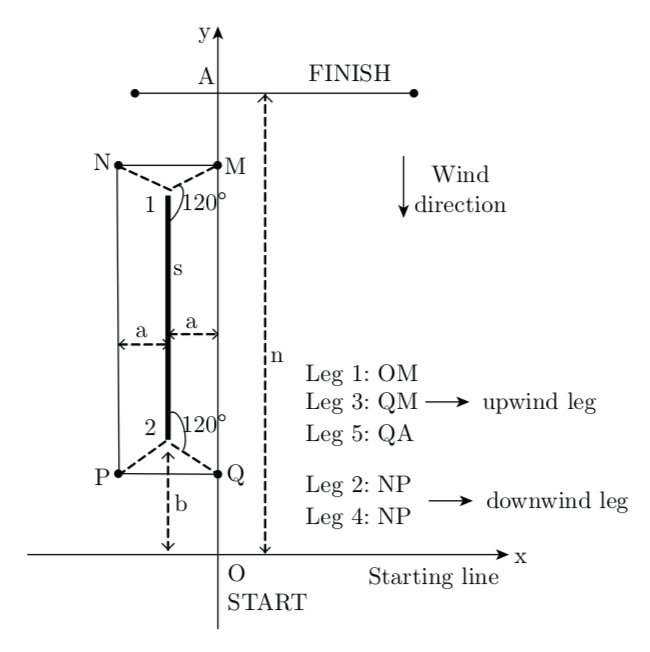
\includegraphics[width=0.5\linewidth]{xiingpath.png}
 \caption{Two-dimensional plane model for upwind-downwind course. The coordinate of bouy 1 is (-a,b+s) and for buoy 2 is (-a,b) \cite{xing2012path} }
\label{xiingfig1}
\end{figure}
In  \cite{xing2012path} how the the start and end lines are defined \ref{tracks} were considered for the developement of the algorith. Then,  the set-up defined is two-dimensional coordinates system with only 2 bouys as shows in figure \ref{xiingfig1}.  Each leg on the course can be represented with this figure with some adjustments. 
%These adjustments were defined as in figure \ref{xiin_relang}.
%\begin{figure}
%\centering
%  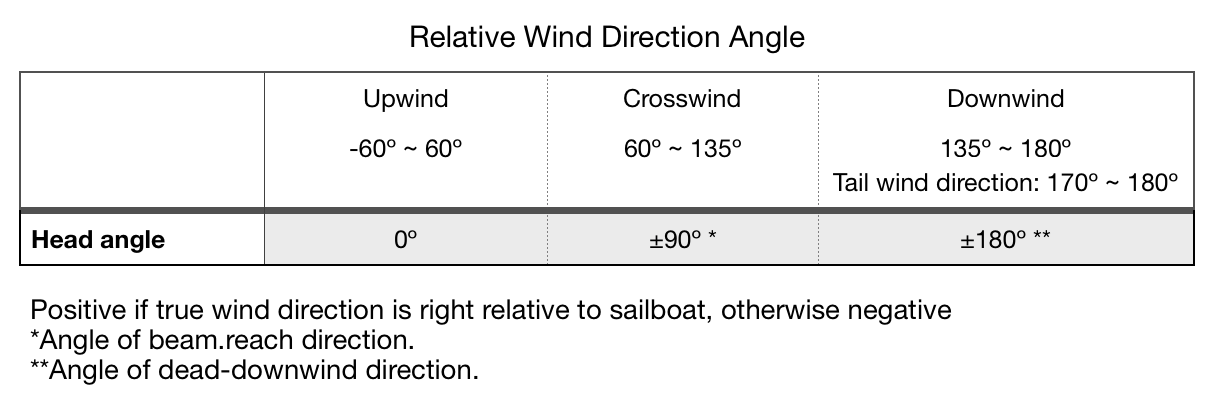
\includegraphics[width=0.7\linewidth]{catrelang.png}
% \caption{Categories on relative wind angles according \cite{xing2012path} }
%\label{xiin_relang}
%\end{figure}
In addition to this, another condition imposed was that center of sailboat follows the line made by the point QM and NP and the connection between the bouy and each of the points (virtual) was defined by imposing a link line with an angle of 120º. In this way, the 180º turns, MN and PQ trajectories, are sailing in beam reach  and with a maximum speed due to the trimming sail angle is approximate 45º, see figure \ref{xiingfig1}. % The coordinates of each of these 4 points are shown in figure  ref{xiingcoord}.\\
%\begin{figure}
%\centering
%  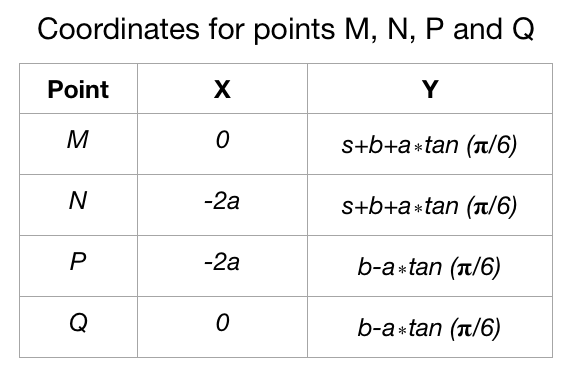
\includegraphics[width=0.5\linewidth]{coord.png}
% \caption{Categories on relative wind angles according \cite{xing2012path} }
%\label{xiingcoord}
%\end{figure}
The whole competition was divided in legs and %that Xing considered includes the star and end lines and the 2 buoys previously explained, then 5 legs were defined.  
for each of these additional legs, the shortest range L was defined.\\ %which is basically the Y coordinate or minimum distance between points see figure   \ref{xiinglegs}.
%\begin{figure}
%\centering
%  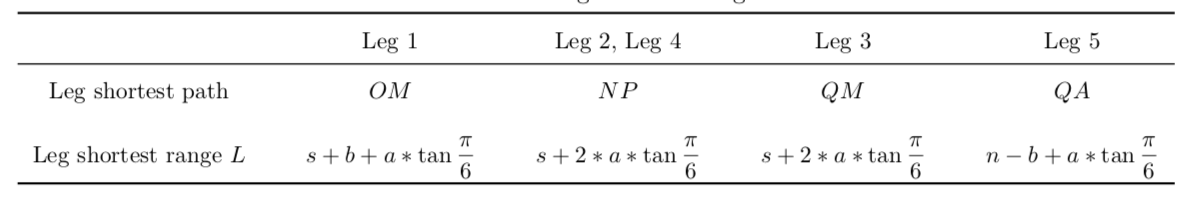
\includegraphics[width=0.8\linewidth]{xinglegs.png}
% \caption{Leg shortest range from \cite{xing2012path} }
%\label{xiinglegs}
%\end{figure}
%Because of the upwind-downwind conditions some coordinates have to be reverting or shifting and the same happens with the angle of the current, $\gamma_{C}^{0}$, and wind $\varphi^{0}$.  The rotation from true direction relative to the each leg coordinate system are illustrated in figure \ref{xiingrel_wc}.\\ 
%\begin{figure}
%\centering
%  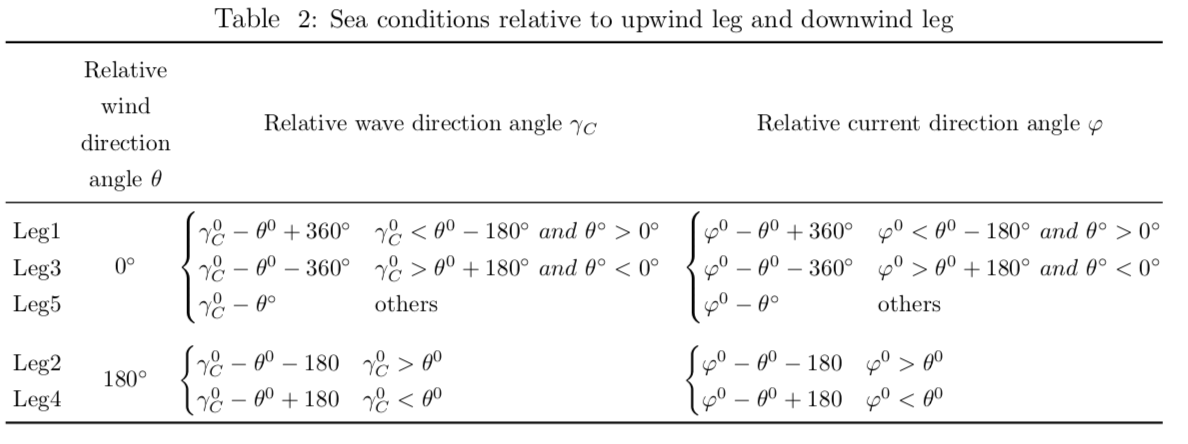
\includegraphics[width=1\linewidth]{xing_rot.png}
% \caption{Conditions relative to upwind leg and downwind leg \cite{xing2012path} }
%\label{xiingrel_wc}
%\end{figure}
%The optimization process  is based on the grid method and heading decision; for this the information was processed by stages or windows represented by each of the legs,  and in each stage the optimal solution was obtained by first inspection the information. *** REVISAR
The optimization process is based on the grid method and heading decision. For this, it was found that the maximum velocity of the boat is at 48º sailing against the wind. Hence at each leg  a fictitious area or window with the shape of a diamond of 50º at each side was defined from the starting point, $P_{0}$, to the target point,$P_{n}$, at y-axis is evenly divided into n sailing sections whose shortest distance is \textit{L/n}. The even \textit{n} was determine based on \textit{L} and the experiences. Xing divide the bottom part of the diamond to get 21 routes followed each by 5º interval clockwise and counterclockwise. Equation \ref{xing_nodesi} is the expression that gives the number of nodes divided on each section its graphical representation is on figure \ref{xing_fignodesi}. 
\begin{equation}
\label{xing_nodesi}
num=
\begin{cases}
20k+1,  & k=0,1,...\nicefrac{n}{2} \\
\\
\noindent 
\displaystyle
20(n-k)+1, & k=\nicefrac{(n+1)}{2}, .... ,n\\
\end{cases}
\end{equation}
\begin{figure}[hbt!]
\centering
  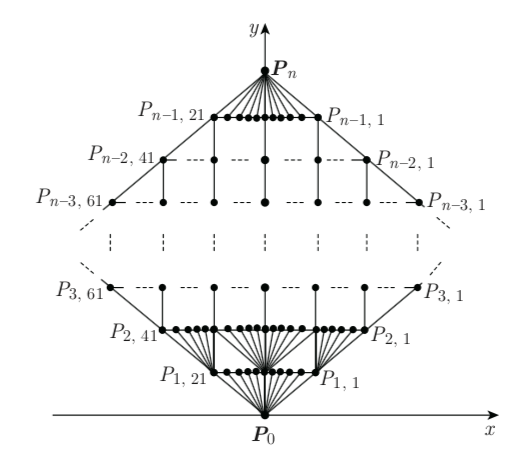
\includegraphics[width=0.6\linewidth]{legyachtxing.png}
 \caption{Leg yatching model \cite{xing2012path} }
\label{xing_fignodesi}
\end{figure}
\begin{equation}\label{evalxing}
EV_{k_j}=\tau_{1}T_{k_j}+\tau_{2}\eta Z(x_{k_j},y_{k_j})
\end{equation}
Each subroutes were evaluted in the $P_{k_j}$ direction of section \textit{k} with a heading decision comprehensive evaluation function $EV_{k_j}$.  Equation  \ref{evalxing}  weights the maximum speed at given heading and the distance to reach the target.
The time is given by $T_{k,j}$  which includes the actual velocity and the distance it takes to reach the objective. In the first part of the equation, the time is weighted while in the second,   $Z(x_{k,j},y_{k,j})$  is the distance to the target point. The weight of each part is defined by $\tau_{i}$, and the value of each part is given according the experience of the sailor, the same happend for $\eta$ which is a negative value because it stands for the how close the boat is sailing towards the target direction.\\
The optimal heading is obtained by finding the minimum of the comprehensive evaluation function of all the 21 headings with the limiting condition of sea-route width M.
\begin{equation}
\label{optheadxing}
\begin{aligned}
f_{k}=min \{EV_{k,j} \}, & &  j \in \{1,2,3,...21\} \\
s.t (M-|x_{k,j}|) > 0
\end{aligned}
\end{equation}
But to find the optimal path on each leg, the algorithm has to search among all the alternatives. Considering the time spent sailing from one node to another and  the time from the start to the node, The criterium for each of this arguments is that it has to be the best time, in other words the minimum time. The time of each route is store and latter compared. At the end the best routes, are connected and the final path is obtained. \\
\subsection{Model: yatch vs dinghy}
The dinghy is one of the smallest boats propelled by wind, with a maximum weight of 59 kg \cite{sailoly}. Therefore its balance, mainly in the heave axis, between the heel angle and righting moment is determine by the ability of the crew to adjust its posture over each side of the boat \cite{marchajaereo1979} as a response of the wind speed and direction to confront.  As mentioned in \cite{philpott1993yacht} and \cite{larsonprinciples} this assumption is implicit in order to keep the analysis in 2D and consequently represented in VPP.  \\
In \cite{day2017performance} a deeper analysis and comparison between the adaptations on the standard VPP were addressed including the  "data taken from the  (Offshore Rating Congress, 2013 )" and the observations made in other works like in  \cite{carrico17symp}, \cite{binns2002development} and \cite{flay1996twisted}. Particularly in \cite{carrico17symp} these modifications correspond to the addition of the \textit{reef} and \textit{flat} coefficients. They account for the fact that dinghy's sails do not reef against strong winds. This condition affect the drag and lift coefficients on the upwind and downwind course. In \cite{day2017performance} the adaptations where divided according  the aerodynamic and hydrodynamic forces, where \textit{flat}, \textit{twist} coefficients and the \textit{spill} variable where included to model the behavior of the sails and athlete under strong wind conditions, in additions to some conditions to be included when a downwind course is sailed. \\
The literature regarding VPP for laser boat classes is limited and it is mainly accounted in \cite{day2017performance}, the comparisons made here are only valid for wind speed between  4 and 16 knots, while races are performed up to 25 knots. This range have to be consider in the developed and validation of the algorithm to find the optimal path since it is the velocity of the wind that determines the direction that should be taken in order to maximize the VMG parameter. \\
\subsection{Weather Integration}
Uncertainty weather is a typical condition that not only yacht competitions  have to manage but also maritime transportation. This type of competitions or courses could take days, weeks or even months; an example of  it is the \textit{Volvo Ocean Race}, which is an around ocean race.  In the case of maritime transportation the approach is to minimize the cost in terms of  fuel consumption, arrival time or increase productivity, the efficiently use of vessels at is minimum cost  (reference). The importance to take good decisions on time depends on: the available data, which provides feedback to the current status or decision and processing time,  how much time the data can be converted in meaningful information. These two variables have been approaching by different researchers to obtain the optimal path specially on maritime and logistics, a less number can be found for yacht races and autonomous vehicles, a just a fewer number refer to Olympic races. \newline
Allsopp \cite{allsopp2000optimal} in his paper \textit{Optimal Sailing Routes with Uncertain Weather} considers not only  the current and wind as time dependent variables  but also the computational time to process new data and determine the optimal path for around ocean races, like he \textit{Volvo Ocean Race}.  As he mentioned most of the available softwares define the optimal path assuming a deterministic approach, which means that the forecast of the weather will come out as it.  Instead of this, he use a stochastic weather approach to contemplate  different weather conditions and its changes to display an optimal route according each set of conditions, in other words he consider a dynamic programing to adapt the route according them.  
First, different wind and current vectors fields were determine, time dependent variables, and included in a VPP plot to determine the boat's velocity at any time and conditions;  which is reached by a lookup function. 
The route was determine by the start, \bm{$x$}$_{start}$,  and finish locations, \bm{$x$}$_{finish}$,  start time $t_{start}$, current  \bm{$c(x,$}t\bm{$)$} and wind fields \bm{$w(x,$} t \bm{$)$}  depend on time and location. By discretizing the race into different nodes, the time to sail from node \textit{i} to \textit{j} can be determine as $c_{arc}$ \textit{(i,j,t(i))} with the next recursion dynamic program \cite{allsopp2000optimal}:
\begin{equation}
\label{Allsopp1eq}
f^*(i,t)=
\begin{cases}
0,  &  \\
\\
\noindent 
\displaystyle
\min_{j \in \Gamma} [ c_{arc}(i,j,t)+f^*(j,t + c_{arc}(i,j,t)) ], & i=n_{finish}\\
\end{cases}
\end{equation}
 \hspace{20mm} otherwise
\begin{equation*}
j^*(i,t)=
\noindent 
\displaystyle
arg \min_{j \in \Gamma} [ c_{arc}(i,j,t)+f^*(j,t + c_{arc}(i,j,t)) ], \quad i \neq n_{finish} 
\end{equation*}
With these equations, the time is minimized at each node until the finish is reach. These state-space of the  shortest path includes explicitly the time dimension which is used in the dynamic program.
 \begin{figure}
\centering
  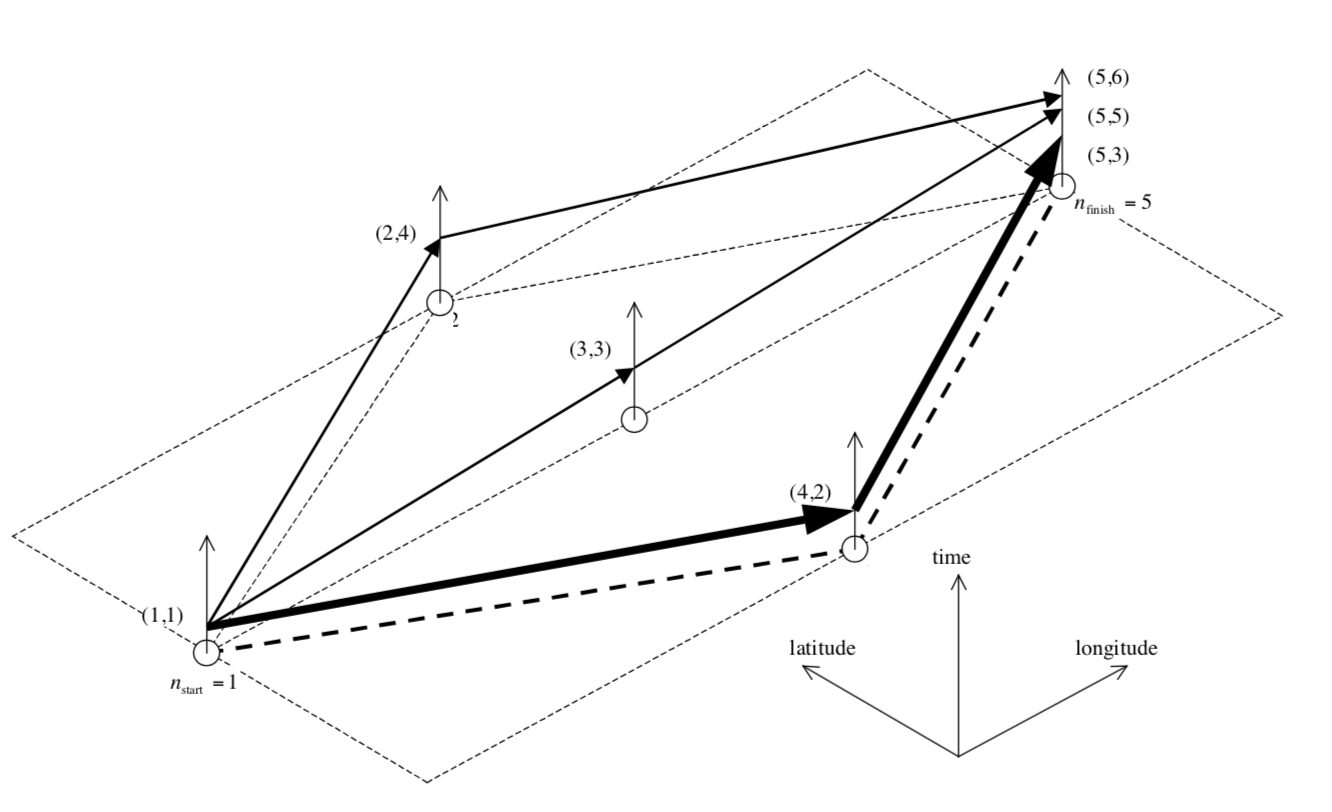
\includegraphics[width=\linewidth]{Allsopp1.png}
 \caption{Deterministic dynamic program with time shown as an explicit state. Nodes (index,time) \cite{allsopp2000optimal} }
\label{Allsopp1fig}
\end{figure}
In the case, of the weather Allsopp \cite{allsopp2000optimal} use the simplest stochastic model to include the uncertainty of the wind speed and direction at each point as a random variable with a known distribution; and use a branching scenario model to incorporate the information about past conditions. 
%Therefore, this structure represents the arrival of new information while each node, the actual information. The assembling of information at each node  is represented as a \textit{bundle B(s,t)}  where s stands for the scenario at time t. 
%\begin{figure}
%\centering
 % 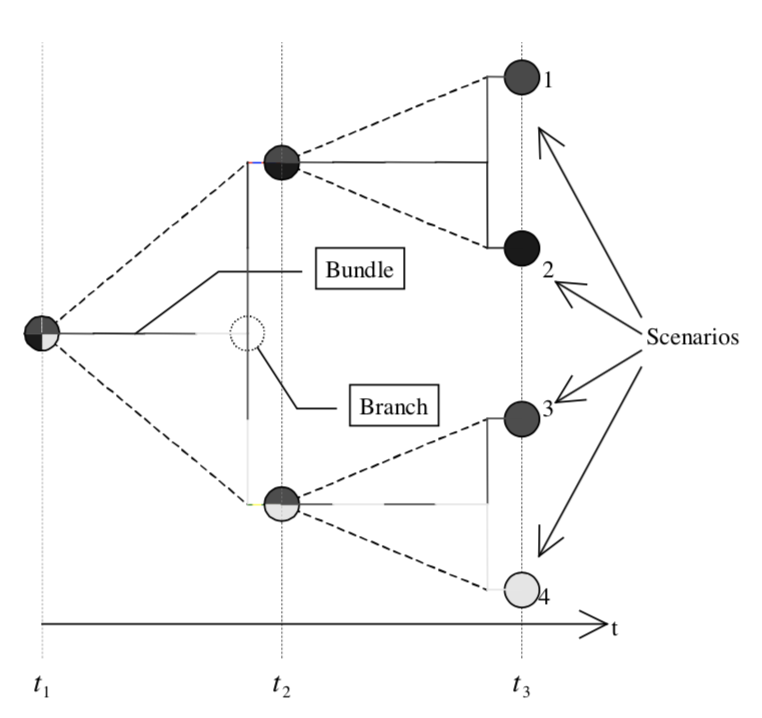
\includegraphics[width=0.6\columnwidth]{Allsopp2.png}
 %\caption{Scenario structure with three branches and four scenarios. Identical scenarios treated as one \textit{bundle} \cite{allsopp2000optimal} }
%\label{Allsopp2}
%\end{figure}
%The uncertainty is included by addition the location in the scenario tree, then the node is represented as \textit{(i,t,s)}. Since the only scenarios that can possibly eventuate are those in the same bundle as \textit{s} at time \textit{t}, $s^'$ $ \in  B(s,t)$.  Then the expected optimal time to go from \textit{i}, at time \textit{t}, in scenario \textit{s}, when passing through node \textit{j} next is given by:
%\begin{equation}
%\label{Allsopp2eq}
%t^*(i,j,t,s)=
%\noindent 
%\displaystyle
%\sum_{s'  \in B(s,t)}  \frac{p_{s'}} {p_{B(s,t)}} [ c_{arc}(i,j,t,s')+f^*(j,t + c_{arc}(i,j,t,s'),s') ]
%\end{equation}
%where $t^*(i,j,t,s)=
%\noindent 
%\displaystyle
%\sum_{s'  \in B(s,t)}  p_{s'}$ is the probability of the bundle containing scenario \textit{s} at time \textit{t} and $\nicefrac {p_{s'}} {p_{B(s,t)}} $  is the conditional probability of scenario \textit{s'} at time \textit{t} given that it is known that one of the scenarios in the bundle containing scenario \textit{s} will eventuate.  Modifying [ \ref{Allsopp1eq} ]   will give the stochastic forward-looking recursion:
%\begin{equation}
%\label{Allsopp3eq}
%f^*(i,t,s)=
%\begin{cases}
%0,  &  \\
%\\
%\noindent 
%\displaystyle
%\min_{j \in \Gamma} t^*(i,j,t,s), & i=n_{finish}\\
%\end{cases}
%\end{equation}
 %\hspace{32mm} &                         otherwise 
%\begin{equation*}
%j^*(i,t,s)=
%\noindent 
%\displaystyle
%arg \min_{j \in \Gamma} t^*(i,j,t,s), \quad i \neq n_{finish} 
%\end{equation*}
%This last equation is the core of the dynamic program we use to obtain the stochastic routes.
%For the implementation of this equation the computational effort or time has been kept. To reduce the running times, the distance between nodes was considered and use bounding to speed-ups, in addition, the successors were excluded based on angle spacing %and distance respectively. Beside the adaptation of Pijavskii-Shubert algorithm for global optimization to achieve a small further speed-up.\par
The distinction between short course races and long course has been considering in the development of methods for the optimal path. The random fluctuation over the time is more sensitive on short courses rather long coursed, because of this Philpott \cite{philpott2001optimising} describe a method for each condition to figure out the optimal path.  The weather variables in a short courses were considered to have a minimum spatial variation, although they enclose a random component due to its dependance over time.\\
This dependency can be expressed with a discrete Markov chain; in other words, the wind intensity \textit{W} and its direction $\theta$ have a Markov chain structure.  Since the boat speed is different  between upwind and downwind, it is recommended to separate each leg or course and adjust $\Delta t$ as necessary. $\Delta t$ remains constant over the leg but it could be change between legs.  %The method that Philpott suggest first define the deterministic version of the problem which is solve with dynamic programing and then it is solve as a stochastic problem.  
The area of sailing is discretize with a rectangular grid, and it defined nodes, so the dynamic  programming can be set. A loss time variable is included to take into account tacked manoeuvres. After setting these parameters and conditions the model has to incorporate the stochastic process into the recursion. % Stochastic variable as utility functions takes into account the risk  attitude which could be risk-averse or risk-seeking, in sailing races to minimize  \textit{T} this means that a risk averse would minimize \textit{u(T)} while a risk-seeking would minimize \textit{v(T)}; \textit{u( )} and \textit{v()} are convex and concave functions respectively. A convex function accentuates large \textit{T} values and discourage them whereas  a concave discourage them by weighting them with a minor proportion of an expected time. 
With this method the area and time have to being discretize, more over the it consider different states or possibles angles at which the wind will be directed. Which means that each location has to evaluate each of the states and find the optimal path among  \textit{n} stages.  The larger or the smaller the the discretization the more locations to solve according each stage, which seem that the computational effort will grow considerably since each leg has to be evaluated.  The paper does not mention the computational effort nor the difference of time that can be achieve by using it.
\subsubsection{Wind Model}
Weather model forecast are calculated  by super computer and updated every three hour according regions. Different agencies have developed models to predict it in global terms. The local prediction are made based on it with via extrapolation and interpolation between local measurements with the intention to predict it every hour, for local purposes. The global and open information is stored in what is know as GRIB or NET files. This files, GRIB, is downloaded according the region of interest the common grid size provides is a 3 km square. 
In \cite{binns2002development} the simulator use a guts wind model  with the next parameters: the time step was defined as 60 seconds and the length of 200 m. It can be said that the grid of the simulation are these paremeters mentioned.
\section{The model: Algorith for the minimal time path}
\section{Validation}
\section{Results}
\section{Discussions and Conclusions}
\appendix
\subsection{Equations } \label{forces_equations} %% ADD information for fossati
%\section{VPP algorithm} \label{vpp_alg} %% add information milgram diagram page 4
\begin{figure}
\centering
  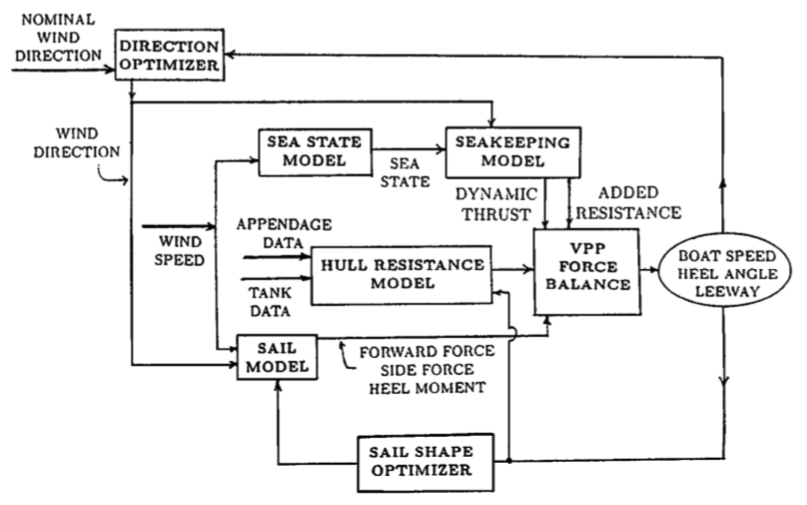
\includegraphics[width=0.8\columnwidth]{vpp_map_milgram.png}
 \caption{A block diagram of the VPP. This emphasize the fact that solving the force balance equation is the minor and more ordinary part of the process. The modeling of the process is necessary imperfect and requires most of the effort in developing a faithfull VPP. \cite{milgram1998fluid} }
\label{vpp_diagram}
\end{figure}
\newpage
%%

In sailing, the motions with respect to the wind define the type of manouvres to execute.  Since the sailboat can not displace towards the wind, tacking manoeuvers are perform. These type of paths are described as zig-zag patterns that can be started on the left- or on the right-hand side. Another condition is dictated when the boat is displaced in the same direction as wind. These conditions shows that feasible paths are asymmetrical\cite{dolinskaya2012optimal}. Because athletes are not allow to get any information or feedback from coaches, preparation is crucial. The information of how to course must be deliver before competition and it have to be trained. Another element to consider is the no-go zone where the propulsion is null or not enough to displace the sailboat\cite{yang2011control}.\par
